\section{Строки.}%


\subsection{Совпадение подстрок в строке.}%

Построим \textbf{полиномиальную} хеш-функцию, которая каждой строке в соответствие ставит число.
\[h_{p, m}(\overline{c_{0}c_{1}...c_{n}}) = (c_0 \cdot p^{n - 1} + c_1 \cdot p^{n-2} + ... + c_{n - 2} \cdot p + c_{n - 1}) \ \% \ m\]

При помощи схемы Горнера, такая функция считается за линейное время, ведь $h_{p, m}(\overline{c_{0}c_{1}...c_{n}}) = (...(((c_0 \cdot p + c_1))p + c_2)p + c_3)...)p + a_{n-1}$

Так как мы имеем дело с подстроками одной большой строки, мы можем сделать предподсчет хеш-функции для всех префиксов большой строки, а дальше воспользоваться свойством хеша:
\[
	h(S[l, r)) = (h(S[0, r)) - h(S[0, l)) \cdot p^{r - l + 1}) \ \% \ m
.\] 

Таким образом, после линейного предподсчета, мы можем сравнивать строки по их хешу за константное время.


\subsection{Алгоритм Рабина -- Карпа для поиска подстроки в строке.}%

Для поиска подстроки $S$ длины $m$ в тексте $T$ длины $n$, 
\begin{enumerate}
	\item Подсчитаем $h(T[0, m))$ и $h(S[0, m))$, а также $p^m$.
	\item В цикле по всем $i$ от  $0$ до $n - m$
		\begin{enumerate}
			\item Считаем $h(T[i, m + i))$ и сравниваем его с $h(S[0, m))$. 
			\item В случае равенства, опционально, можно провести проверку наивным посимвольным сравнением или выборочным сравнением символов, для исключения малейшей вероятности коллизии.
		\end{enumerate}
\end{enumerate}

Алгоритм работает за линейное время $O(n + m)$, однако он не устойчив перед коллизиями хеш-функции, дополнительная обработка которых увеличивает время работы.


\subsection{Алгоритм Кнута -- Морриса -- Пратта для поиска подстроки в строке.}%

\subsubsection{Префикс-функция}
Введем для строки $S$ префикс-функцию $\pi$ 
\[
	\pi(i) = \max \limits_{k \in [0, i]} \{k: S[0, k) == S[i + 1 - k, i +1)\}
\]
-- длина наибольшего собственного суффикса подстроки S[:i], который равен префиксу такой же длины. $\pi(0) = 0$ по определению.

\begin{example}
	$S = "adam"$. 
	$\pi(0) = 0$. \\
	$\pi(1) = 0$, ведь у строки  $"a"$ есть только пустой собственный суффикс. \\
	$\pi(2) = 0$, ведь у строки $"ab"$ нет собственного суффикса, совпадающего с префиксом той же длины. \\
	$\pi(3) = 1$, ведь у строки  $"ada"$ есть собственный суффикс  $"a"$ длины 1, который совпадает с префиксом  $"a"$. \\
	$\pi(4) = 0$. \\
\end{example}

Нетрудно представить себе наивный алгоритм, подсчитывающий префикс-функцию строки за $O(n^3)$. Оптимизируем его.



 \begin{prop}
	 $\pi(i + 1) \leq \pi(i) + 1$
\end{prop}
\begin{proof}
	Рассмотрим суффикс, оканчивающийся на позиции $i + 1$ и имеющий длину $\pi(i + 1)$. Удалив из него последний элемент, мы получим суффикс, оканчивающийся на позиции $i$ и имеющий длину  $\pi(i + 1) - 1$\\
	Однако, мы определили $\pi(i)$ максимальную длину суфикса  $\Rightarrow$ $\pi(i) \geq \pi(i + 1) - 1$.
	\begin{center}
		\framebox{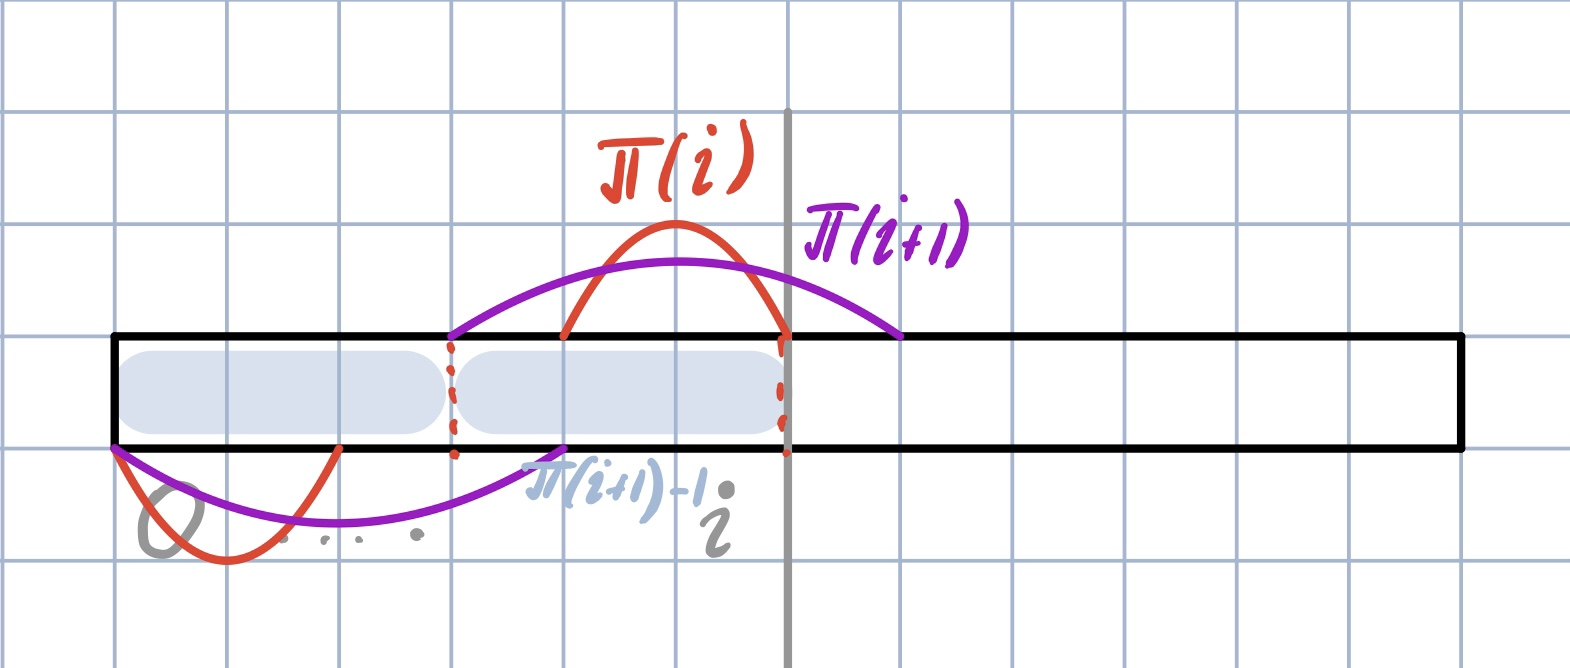
\includegraphics[scale = 0.1]{~/Study/3rdSem/Algorithms/Abstracts/images/lect05/dec_pi_leq.jpeg}}
	\end{center}
\end{proof}

\begin{prop}
	Если $S[\pi(i)] == S[i + 1]$, то  $\pi(i + 1) == \pi(i) + 1$.
\end{prop}
\begin{proof}
	Условие говорит нам, что после префикса длины $\pi(i)$ находится символ, который совпадает с символом, который находится после суффикса, оканчивающегося на позиции $i$. То есть наибольший суффикс, заканчивающийся на позиции $i + 1$ содержит в себе все символы суффикса, заканчивающегося на позиции $i$ и еще один символ. Это и записано в правой части.
	\begin{center}
		\framebox{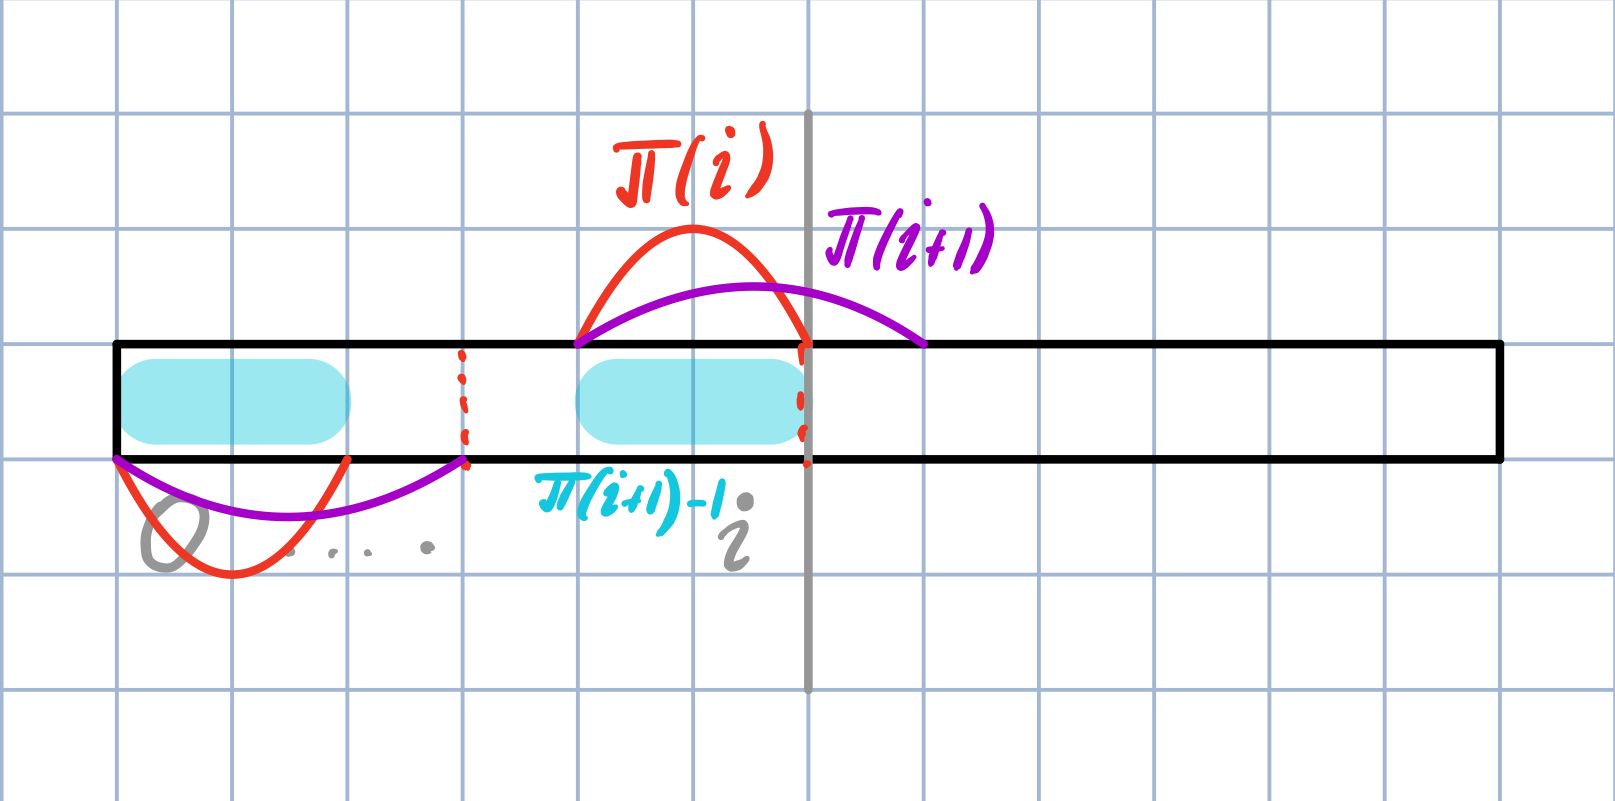
\includegraphics[scale = 0.1]{~/Study/3rdSem/Algorithms/Abstracts/images/lect05/dec_pi_i_plus_1.jpeg}}
	\end{center}
\end{proof}

Пользуясь вторым свойством, мы сможем частично оптимизировать подсчет. Если же окажется что условие равенства символов не выполняется, мы будем искать суффикс меньшей длины следующим образом:
Мы знаем, что $S[1, \pi(\pi(i)))$ -- суффикс подстроки  $S[1, i)$ \\

\textbf{Тогда подсчет можно свести к циклу}
\begin{enumerate}
\setcounter{enumi}{0}
	\item $k = \pi(i)$.
	\begin{enumerate}
		\item Если $S[i + 1] == S[k]$, то $\pi(i + 1) = k + 1$.
		\item Если же $k == 0$, то $\pi(i + 1) = 0$.
	\end{enumerate}
	\item $k = \pi(k)$. Перейти к пункту 1.
\end{enumerate}

Теперь мы будем проходиться по строке, и для каждой позиции вычислять $\pi(i)$ оптимизированно.

\begin{prop}
	Оптимизированный алгоритм подсчета префикс-функции имеет асимптотику $O(n)$.	
\end{prop}
\begin{proof}
	Из вышедоказанного утверждения мы знает что на каждой итерации по индексу строки, $k$ увеличивается не более чем на 1.
\end{proof}

\subsubsection{Z-функция}

Введем для строки $S$ Z-функцию $z$ 
\[
	z(i) = \max \{k: S[i, i + k) == S[0, k)\}
\]
-- длина наибольшей подстроки S, начинающейся с позиции $i$, которая равна префиксу S такой же длины, $z(0) = 0$ по определению.

\begin{example}
	$S = "adam"$. 
	$z(0) = 0.$
	$z(1) = 0.$
	$z(2) = 1.$ 
	$z(3) = 0.$
\end{example}

\begin{Def}
	\textbf{Z-блок} --- подстрока $S$, начинающаяся с позиции  $i$ длины  $z(i)$.
\end{Def}

\textbf{Для построения Z-функции} строки $S$ будем на каждом шаге хранить самый правый  Z-блок -- тот, у которого правая граница является самой правой.
Назовем позиции начала и конца самого правого Z-блока $l$ и  $r$ соответственно. Изначально $l = r = 0$. 

Пусть у нас подсчитана Z-функция и Z-блок для всех позиций $< i$, тогда найдем  $z(i)$.

Рассмотрим 2 случая. 
\begin{enumerate}
	\item \underline{$i \notin [l; r)$}: \\
		Тогда нам придется считать функцию наивно, пробегая двумя указателями по строке с начала и по подстроке, начиная с позиции $i$. Тогда значение $z(i)$ будет определено как первая позиция $j$, такая что  $S[j] != S[i + j]$.
		После этого обновим сохраненное значение самого правого Z-блока.
	\item \underline{$i \in [l, r)$}: \\
		Тут возможны 2 варианта:
		\begin{enumerate}
			\item \underline{$z(i - l) < r - l$}. То есть наибольшая подстрока, начинающаяся с позиции $i - l$, равная префиксу такой же длины, не превышает по длине самый правый Z-блок. \\
				Заметим, что позиция $i - l$ будет лежать в префиксе, равном по длине самый правый Z-блоку. \\
				Тогда $z(i) = z(i - l)$. \\
		\item \underline{$z(i - l) > r - l$}. В этом случае наибольшая подстрока, начинающаяся с позиции $i - l$ выходит за пределы префикса, соответствующего самому правому Z-блоку. \\
				Тогда скажем  что $z(i) = r - i + l$ --- длина той части наибольшей подстроки, начинающейся с позиции  $i - l$, которая лежит внутри префикса, соответствующего самому правому Z-блоку. \textbf{А затем будем наивно улучшать оценку, проходясь по строке начиная с позиции r.}
		\end{enumerate}
\end{enumerate}

\begin{prop}
	Асимптотика вычисления Z-функции --- $O(m)$, где $m$ --- длина строки.
\end{prop}
\begin{proof}
	Каждая позиция в строке просматривается не более двух раз. При попадании в промежуток $[l; r)$ и наивном улучшении, или же в противном случае при непопадании в промежуток и наивном просчете. При этом, всякий раз когда мы считаем Z-функцию наивно, мы обновляем самый правый Z-блок, то есть сдвигаем его правую границу, а это может происходить не более $m$ раз. Значит мы тратим $O(m)$ на базовые операции и $O(m)$ на суммарные наивные проверки.
\end{proof}

\newpage

\subsubsection{Алгоритм}
Для поиска подстроки $S$ длины $m$ в тексте  $T$:
\begin{enumerate}
	\item Построим строки вида $S\#T$, где $\#$ --- произвольный разделитель, не встречающийся в тексте.
	\item По сконструированной строке построим префикс-функцию или Z-функцию.
	\item Тогда если в некоторой позиции  $i$ $\pi(i) == m$, то эта позиции --- конец вхождения подстроки. \\
		Аналогично, если $z(i) == m$, то эта позиция --- начало вхождения подстроки.
\end{enumerate}

\begin{prop}
	Алгоритм работает за $(\lvert S \rvert + \lvert T \rvert)$.
\end{prop}
\begin{proof}
	Ведь Префикс-функция и Z-функция строятся за линейное время, а затем совершается только один проход всей результирующей строки.	
\end{proof}
